%!TEX root = ../template.tex
%%%%%%%%%%%%%%%%%%%%%%%%%%%%%%%%%%%%%%%%%%%%%%%%%%%%%%%%%%%%%%%%%%%%
%% chapter5.tex
%% NOVA thesis document file
%%
%% Chapter with lots of dummy text
%%%%%%%%%%%%%%%%%%%%%%%%%%%%%%%%%%%%%%%%%%%%%%%%%%%%%%%%%%%%%%%%%%%%

\typeout{NT FILE chapter5.tex}%

\chapter{Ant Colony System di Dorigo et al}\label{chapt:5}



\section{Fondamenti}

\subsection{Ispirazione Biologica}
L'Ant Colony System (\Gls{ACS}) trae ispirazione delle formiche reali, che possono trovare in modo efficiente i percorsi più brevi tra le fonti di cibo e il loro nido. Questa capacità è attribuita ai sentieri di feromoni tracciati dalle formiche, facilitando una forma indiretta di comunicazione che guida altre formiche verso percorsi ottimali\cite{Dorigo1996, Dorigo1997}.

La stigmergia, un meccanismo di coordinazione indiretta tra agenti, gioca un ruolo cruciale in questo processo\cite{Bonabeau1999}. Le formiche depositano feromoni mentre si muovono, creando un feedback positivo che rafforza i percorsi più efficienti nel tempo\cite{Deneubourg1990}.

\subsection{Principi Algoritmici}
L'\Gls{ACS} sfrutta una colonia di formiche artificiali che lavorano cooperativamente per esplorare e sfruttare soluzioni per problemi di ottimizzazione. L'approccio integra sia l'esplorazione di nuove soluzioni sia lo sfruttamento di soluzioni buone conosciute attraverso un equilibrio tra l'influenza dei feromoni e la desiderabilità euristica.\cite{Dorigo1996, Dorigo1997}

Dorigo et al. hanno introdotto diversi miglioramenti rispetto agli algoritmi precedenti basati sulle formiche:

\begin{itemize}
	\item Una regola di transizione di stato più forte che bilancia meglio l'esplorazione di nuovi archi e lo sfruttamento della conoscenza accumulata sui problemi.
	\item Una regola di aggiornamento globale dei feromoni applicata solo agli archi appartenenti al miglior tour.
	\item L'applicazione di una regola di aggiornamento locale dei feromoni durante la costruzione delle soluzioni.
\end{itemize}

\begin{figure}[]
	\centering
	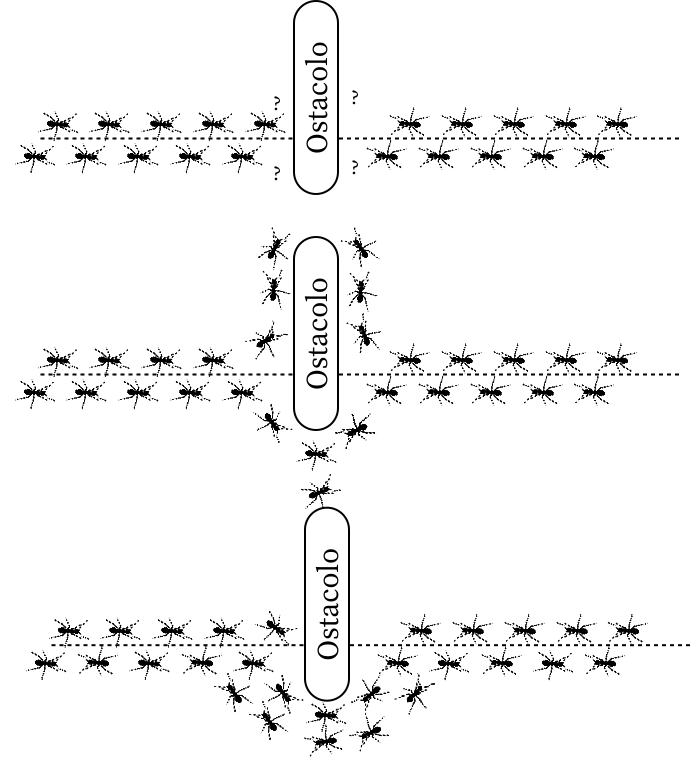
\includegraphics[width=0.7\textwidth]{Chapters/Figures/ants_path.png}
	\caption{Comportamento delle formiche di fronte ad un ostacolo}
	\label{fig:obstacle}
\end{figure}

Nella figura ~\ref{fig:obstacle}
\begin{enumerate}
	\item Le formiche scelgono randomicamente tra i percorsi disponibili
	\item Poiché le formiche si muovono a una velocità approssimativamente costante, quelle che scelgono il percorso inferiore, più corto, raggiungono il punto di decisione opposto più velocemente di quelle che scelgono il percorso superiore, più lungo.
	\item  Il feromone si accumula a un ritmo più elevato sul percorso più breve. Le formiche scelgono il percorso inferiore in base alla concentrazione di feromone.
\end{enumerate}


\subsection{Applicazione al \Gls{TSP}}
Il \Gls{TSP} è particolarmente adatto per l'applicazione dell'\Gls{ACS} a causa della sua necessità di soluzioni efficienti per la ricerca di percorsi. L'algoritmo simula il comportamento delle formiche per costruire percorsi, con il processo di ottimizzazione guidato sia da informazioni euristiche (ad es., distanze tra le città) sia da sentieri di feromoni che rappresentano una forma di esperienza appresa\cite{Dorigo1997, Gambardella1995}.

Nel contesto del \Gls{TSP}, ogni formica costruisce un tour visitando tutte le città esattamente una volta. La scelta della prossima città da visitare è influenzata sia dalla distanza (informazione euristica) che dalla quantità di feromoni sull'arco che collega le città (esperienza accumulata).

\section{Dettagli implementativi}

\subsection{Regole di Aggiornamento dei Feromoni}

Le regole di aggiornamento dei feromoni nell'\Gls{ACS} sono cruciali per guidare il processo di ricerca verso aree promettenti dello spazio delle soluzioni. Queste regole sono suddivise in aggiornamenti locali e globali.

\subsubsection{Regola di Aggiornamento Locale}
Ogni volta che una formica attraversa un arco $(i,j)$, applica la regola di aggiornamento locale dei feromoni per diminuire il livello di feromoni, incoraggiando l'esplorazione da parte di altre formiche. La regola di aggiornamento locale è data da:
\[
	\tau_{ij} = (1 - \rho) \cdot \tau_{ij} + \rho \cdot \tau_0
\]
dove $\tau_{ij}$ è la concentrazione di feromoni sull'arco $(i,j)$, $\rho$ è il tasso di evaporazione locale (0 < $\rho$ < 1) e $\tau_0$ è il livello iniziale di feromoni.

L'effetto di questa regola è di ridurre la quantità di feromoni su un arco visitato, rendendo quell'arco meno desiderabile per le formiche successive. Ciò aumenta l'esplorazione di percorsi alternativi e aiuta a prevenire la stagnazione precoce su soluzioni subottimali.

\subsubsection{Regola di Aggiornamento Globale}
Dopo che tutte le formiche hanno completato i loro tour, viene applicata la regola di aggiornamento globale agli archi che appartengono al miglior tour (sia globalmente che nell'iterazione corrente). L'aggiornamento globale migliora il sentiero di feromoni sui percorsi critici, rendendoli più attraenti per le formiche future. La regola di aggiornamento globale è definita come:
\[
	\tau_{ij} = (1 - \alpha) \cdot \tau_{ij} + \alpha \cdot \Delta \tau_{ij}^{\text{best}}
\]
dove $\alpha$ è il tasso di evaporazione globale (0 < $\alpha$ < 1) e $\Delta \tau_{ij}^{\text{best}}$ rappresenta i feromoni depositati dalla migliore formica, definito come:
\[
	\Delta \tau_{ij}^{\text{best}} = \begin{cases}
		(L_{\text{best}})^{-1} & \text{se }(i,j)\text{ appartiene al miglior tour} \\
		0                      & \text{altrimenti}
	\end{cases}
\]
dove $L_{\text{best}}$ è la lunghezza del miglior tour.

Questa regola intensifica i feromoni sui percorsi che hanno portato alle migliori soluzioni, guidando la ricerca verso regioni promettenti dello spazio delle soluzioni.

\subsection{Regole di Movimento delle Formiche}

Le formiche selezionano la prossima città da visitare basandosi su una regola decisionale probabilistica che bilancia l'esplorazione di nuovi percorsi con lo sfruttamento dei sentieri di feromoni e delle informazioni euristiche.

\subsubsection{Regola di Transizione}
In \Gls{ACS} la scelta della prossima città da visitare è governata dalla regola di transizione pseudo-casuale-proporzionale. Data una formica $k$ nella città $i$, la probabilità di muoversi verso la città $j$ è determinata da:

\[
	j = \begin{cases}
		\arg\max_{l \in N_i^k} \{[\tau_{il}] \cdot [\eta_{il}]^\beta\} & \text{se }q \leq q_0 \text{ (sfruttamento)} \\
		J                                                              & \text{altrimenti (esplorazione bilanciata)}
	\end{cases}
\]

dove $q$ è un numero casuale uniformemente distribuito in $[0,1]$, $q_0$ è un parametro ($0 \le q_0 \le 1$) che determina il bilanciamento tra sfruttamento ed esplorazione, $\tau_{il}$ è la quantità di feromoni sull'arco $(i,l)$, $\eta_{il}$ è il valore euristico (solitamente l'inverso della distanza), $\beta$ è un parametro che controlla l'importanza relativa dell'informazione euristica, e $N_i^k$ è l'insieme delle città non ancora visitate dalla formica $k$ posizionata nella città $i$.

$J$ è una città casuale scelta secondo la distribuzione di probabilità:

\[
	p_{ij}^k = \frac{[\tau_{ij}] \cdot [\eta_{ij}]^\beta}{\sum_{l \in N_i^k} [\tau_{il}] \cdot [\eta_{il}]^\beta}
\]

Questa regola di transizione favorisce lo sfruttamento delle informazioni accumulate (quando $q \leq q_0$) ma lascia spazio all'esplorazione (quando $q > q_0$).


\begin{table}
	\centering
	\caption{Risultati dell'algoritmo ACS}
	\begin{tabular}{lrrrr}
		\toprule
		Istanza  & Tempo (ms) & Lunghezza Tour & Lunghezza ottima & Gap   \\
		\midrule
		eil51    & 17083      & 434.91         & 426.00           & 2.09  \\
		berlin52 & 18411      & 7606.66        & 7542.00          & 0.86  \\
		eil76    & 33136      & 554.04         & 538.00           & 2.98  \\
		d198     & 94445      & 16584.44       & 15780.00         & 5.10  \\
		lin105   & 123877     & 14981.78       & 14379.00         & 4.19  \\
		pr124    & 292446     & 60760.86       & 59030.00         & 2.93  \\
		lin318   & 338493     & 46646.52       & 42029.00         & 10.99 \\
		u574     & 452117     & 42512.54       & 36905.00         & 15.19 \\
		fl1577   & 2880286    & 25939.85       & 22249.00         & 16.59 \\
		rl5915   & 35872198   & 706188.19      & 565530.00        & 24.87 \\
		\bottomrule
	\end{tabular}
\end{table}
\subsection{Pseudocodice}

\begin{algorithm}[H]
	\floatname{ACS}{}
	\caption{\Gls{ACS} per il \Gls{TSP}}
	\begin{algorithmic}[1]
		\State Inizializza i livelli di feromoni $\tau_{ij} = \tau_0$ per tutti gli archi $(i,j)$
		\State Inizializza la migliore soluzione globale $S_{gb}$ e la sua lunghezza $L_{gb}$
		\For{ogni iterazione}
		\For{ogni formica $k = 1, \ldots, m$}
		\State Posiziona la formica $k$ su una città di partenza casuale
		\State Inizializza il tour parziale $S_k = \emptyset$
		\Repeat
		\State Seleziona la prossima città $j$ usando la regola di transizione
		\State Aggiungi $(i,j)$ a $S_k$
		\State Applica l'aggiornamento locale dei feromoni a $(i,j)$
		\State $i \gets j$
		\Until{il tour $S_k$ è completo}
		\If{$L(S_k) < L_{gb}$}
		\State $S_{gb} \gets S_k$
		\State $L_{gb} \gets L(S_k)$
		\EndIf
		\EndFor
		\State Applica l'aggiornamento globale dei feromoni al miglior tour $S_{gb}$
		\EndFor
		\State \Return la migliore soluzione trovata $S_{gb}$
	\end{algorithmic}
	\label{alg:acs}
\end{algorithm}



\subsection{Analisi della Complessità}
La complessità temporale dell'\Gls{ACS} per iterazione è O($n^2m$), dove $n$ è il numero di città e $m$ è il numero di formiche. Tuttavia, il numero di iterazioni necessarie per la convergenza può variare significativamente a seconda delle caratteristiche del problema e dei parametri dell'algoritmo.

\subsection{Parametri Chiave e loro Impatto}
L'efficacia dell'\Gls{ACS} dipende in modo cruciale dalla corretta impostazione di diversi parametri:

\begin{itemize}
	\item $\rho$: Tasso di evaporazione locale dei feromoni
	\item $\alpha$: Tasso di evaporazione globale dei feromoni
	\item $\beta$: Importanza relativa dell'informazione euristica
	\item $q_0$: Bilanciamento tra sfruttamento ed esplorazione
	\item $m$: Numero di formiche
	\item $\tau_0$: Livello iniziale di feromoni
\end{itemize}

La scelta ottimale di questi parametri può variare a seconda del problema specifico e richiede spesso una fase di tuning.

\section{Varianti e Estensioni}

Dalla pubblicazione originale dell' \Gls{ACS} sono state proposte numerose varianti e estensioni:
\begin{itemize}
	\item MAX-MIN Ant System (\Gls{MMAS}): Introdotto da Stützle e Hoos, \Gls{MMAS} limita i valori dei feromoni entro un intervallo predefinito per prevenire la stagnazione prematura. \cite{Stuetzle1997}
	\item Rank-Base Ant System (\Gls{ASrank}): In questa variante, le formiche sono classificate in base alla qualità delle loro soluzioni, e la quanità dei fermoni depositati è proporzionale al rango.
	\item ACS Ibridi: Combinazioni dell'ACS con altre tecniche di ottimizzazione, come algoritmi genetici o Tabu Search, hanno mostrato risultati promettenti su vari problemi di ottimizzazione combinatoria.
\end{itemize}

\section{Applicazioni oltre il \Gls{TSP}}

Sebbene inizialmente sviluppato per il \Gls{TSP}, l'\Gls{ACS} e le sue varianti hanno trovato applicazioni in una vasta gamma di domini:

\begin{itemize}
	\item Problemi di routing di veicoli
	\item Scheduling e pianificazione
	\item Assegnazione di frequenze nelle reti di telecomunicazione
	\item Bioinformatica e folding delle proteine
	\item Ottimizzazione di reti e grid computing
	\item Problemi di ottimizzazione multi-obiettivo
\end{itemize}

La versatilità dell'\Gls{ACS} lo rende un approccio potente per affrontare problemi complessi di ottimizzazione in vari campi dell'ingegneria e della scienza.
